\documentclass[10pt]{article}

\usepackage[margin=1in]{geometry}
\usepackage{amsmath}
\usepackage{graphicx}
\usepackage{booktabs}
\usepackage{hyperref}
\usepackage{enumitem}
\usepackage{float}
\usepackage[section]{placeins}

\setlist[itemize]{noitemsep,topsep=2pt,leftmargin=1.3em}
\setlist[enumerate]{noitemsep,topsep=2pt,leftmargin=1.5em}

\makeatletter
\renewenvironment{abstract}{\noindent\textbf{Abstract.}\ }{\par}
\makeatother

\title{A Rust BBHash-Style Minimal Perfect Hash Function for Static Lookup Workloads}
\author{Devanshu Singhvi\\
\small UTORid: singhv67}
\date{\today}
% Generated by scripts/generate_paper_numbers.py. Do not edit by hand.
% Generated at 2026-04-16T01:16:46.664075+00:00
% Sources: serial-fixed.csv, serial-auto.csv, serial-keymode.csv, serial-fastrange.csv, bits_per_key.csv
\newcommand{\PaperAutoBuildBetterWins}{103}
\newcommand{\PaperAutoBuildMedianSlowdownPct}{0.13}
\newcommand{\PaperAutoBuildWorseWins}{105}
\newcommand{\PaperAutoComparisonCellCount}{208}
\newcommand{\PaperAutoLookupBetterWins}{156}
\newcommand{\PaperAutoLookupMedianAdvantagePct}{2.21}
\newcommand{\PaperAutoLookupWorseWins}{52}
\newcommand{\PaperBitsGammaEightBetterNFour}{3.9514}
\newcommand{\PaperBitsGammaEightBetterNOne}{4.0586}
\newcommand{\PaperBitsGammaEightBetterNThree}{3.9576}
\newcommand{\PaperBitsGammaEightBetterNTwo}{3.9958}
\newcommand{\PaperBitsGammaEightCppNFour}{3.9505}
\newcommand{\PaperBitsGammaEightCppNOne}{4.0361}
\newcommand{\PaperBitsGammaEightCppNThree}{3.9534}
\newcommand{\PaperBitsGammaEightCppNTwo}{3.9697}
\newcommand{\PaperBitsGammaEightLabel}{2.25}
\newcommand{\PaperBitsGammaFiveBetterNFour}{3.4067}
\newcommand{\PaperBitsGammaFiveBetterNOne}{3.5908}
\newcommand{\PaperBitsGammaFiveBetterNThree}{3.4116}
\newcommand{\PaperBitsGammaFiveBetterNTwo}{3.4487}
\newcommand{\PaperBitsGammaFiveCppNFour}{3.4055}
\newcommand{\PaperBitsGammaFiveCppNOne}{3.4902}
\newcommand{\PaperBitsGammaFiveCppNThree}{3.4082}
\newcommand{\PaperBitsGammaFiveCppNTwo}{3.4248}
\newcommand{\PaperBitsGammaFiveLabel}{1.65}
\newcommand{\PaperBitsGammaFourBetterNFour}{3.2911}
\newcommand{\PaperBitsGammaFourBetterNOne}{3.4590}
\newcommand{\PaperBitsGammaFourBetterNThree}{3.2946}
\newcommand{\PaperBitsGammaFourBetterNTwo}{3.3323}
\newcommand{\PaperBitsGammaFourCppNFour}{3.2894}
\newcommand{\PaperBitsGammaFourCppNOne}{3.3730}
\newcommand{\PaperBitsGammaFourCppNThree}{3.2921}
\newcommand{\PaperBitsGammaFourCppNTwo}{3.3083}
\newcommand{\PaperBitsGammaFourLabel}{1.50}
\newcommand{\PaperBitsGammaNineBetterNFour}{4.2002}
\newcommand{\PaperBitsGammaNineBetterNOne}{4.2959}
\newcommand{\PaperBitsGammaNineBetterNThree}{4.2064}
\newcommand{\PaperBitsGammaNineBetterNTwo}{4.2117}
\newcommand{\PaperBitsGammaNineCppNFour}{4.1986}
\newcommand{\PaperBitsGammaNineCppNOne}{4.2852}
\newcommand{\PaperBitsGammaNineCppNThree}{4.2012}
\newcommand{\PaperBitsGammaNineCppNTwo}{4.2178}
\newcommand{\PaperBitsGammaNineLabel}{2.50}
\newcommand{\PaperBitsGammaOneBetterNFour}{3.0957}
\newcommand{\PaperBitsGammaOneBetterNOne}{3.2744}
\newcommand{\PaperBitsGammaOneBetterNThree}{3.1075}
\newcommand{\PaperBitsGammaOneBetterNTwo}{3.1279}
\newcommand{\PaperBitsGammaOneCppNFour}{3.0892}
\newcommand{\PaperBitsGammaOneCppNOne}{3.1699}
\newcommand{\PaperBitsGammaOneCppNThree}{3.0917}
\newcommand{\PaperBitsGammaOneCppNTwo}{3.7534}
\newcommand{\PaperBitsGammaOneLabel}{1.15}
\newcommand{\PaperBitsGammaSevenBetterNFour}{3.7141}
\newcommand{\PaperBitsGammaSevenBetterNOne}{3.8213}
\newcommand{\PaperBitsGammaSevenBetterNThree}{3.7208}
\newcommand{\PaperBitsGammaSevenBetterNTwo}{3.7563}
\newcommand{\PaperBitsGammaSevenCppNFour}{3.7123}
\newcommand{\PaperBitsGammaSevenCppNOne}{3.7988}
\newcommand{\PaperBitsGammaSevenCppNThree}{3.7151}
\newcommand{\PaperBitsGammaSevenCppNTwo}{3.7314}
\newcommand{\PaperBitsGammaSevenLabel}{2.00}
\newcommand{\PaperBitsGammaSixBetterNFour}{3.5339}
\newcommand{\PaperBitsGammaSixBetterNOne}{3.7227}
\newcommand{\PaperBitsGammaSixBetterNThree}{3.5385}
\newcommand{\PaperBitsGammaSixBetterNTwo}{3.5740}
\newcommand{\PaperBitsGammaSixCppNFour}{3.5320}
\newcommand{\PaperBitsGammaSixCppNOne}{3.6152}
\newcommand{\PaperBitsGammaSixCppNThree}{3.5347}
\newcommand{\PaperBitsGammaSixCppNTwo}{3.5510}
\newcommand{\PaperBitsGammaSixLabel}{1.80}
\newcommand{\PaperBitsGammaThreeBetterNFour}{3.1876}
\newcommand{\PaperBitsGammaThreeBetterNOne}{3.3711}
\newcommand{\PaperBitsGammaThreeBetterNThree}{3.1935}
\newcommand{\PaperBitsGammaThreeBetterNTwo}{3.2290}
\newcommand{\PaperBitsGammaThreeCppNFour}{3.1881}
\newcommand{\PaperBitsGammaThreeCppNOne}{3.2725}
\newcommand{\PaperBitsGammaThreeCppNThree}{3.1907}
\newcommand{\PaperBitsGammaThreeCppNTwo}{3.2073}
\newcommand{\PaperBitsGammaThreeLabel}{1.35}
\newcommand{\PaperBitsGammaTwoBetterNFour}{3.1366}
\newcommand{\PaperBitsGammaTwoBetterNOne}{3.3096}
\newcommand{\PaperBitsGammaTwoBetterNThree}{3.1396}
\newcommand{\PaperBitsGammaTwoBetterNTwo}{3.1741}
\newcommand{\PaperBitsGammaTwoCppNFour}{3.1321}
\newcommand{\PaperBitsGammaTwoCppNOne}{3.2119}
\newcommand{\PaperBitsGammaTwoCppNThree}{3.1347}
\newcommand{\PaperBitsGammaTwoCppNTwo}{3.3668}
\newcommand{\PaperBitsGammaTwoLabel}{1.25}
\newcommand{\PaperBitsTableNFour}{2{,}097{,}152}
\newcommand{\PaperBitsTableNOne}{65{,}536}
\newcommand{\PaperBitsTableNThree}{1{,}048{,}576}
\newcommand{\PaperBitsTableNTwo}{262{,}144}
\newcommand{\PaperCollapsedCellCount}{117}
\newcommand{\PaperFastRangeBuildHighThirtyTwoWins}{19}
\newcommand{\PaperFastRangeBuildLowThirtyTwoWins}{44}
\newcommand{\PaperFastRangeBuildMulSixtyFourWins}{54}
\newcommand{\PaperFastRangeHighThirtyTwoBuildImprovePct}{5.9}
\newcommand{\PaperFastRangeHighThirtyTwoLookupPenaltyPct}{1.8}
\newcommand{\PaperFastRangeLookupHighThirtyTwoWins}{11}
\newcommand{\PaperFastRangeLookupLowThirtyTwoWins}{45}
\newcommand{\PaperFastRangeLookupMulSixtyFourWins}{61}
\newcommand{\PaperFastRangeMulSixtyFourBuildImprovePct}{7.4}
\newcommand{\PaperFastRangeMulSixtyFourLookupImprovePct}{0.2}
\newcommand{\PaperFixedBuildBetterWins}{1250}
\newcommand{\PaperFixedBuildBoomWins}{622}
\newcommand{\PaperFixedBuildTieCount}{0}
\newcommand{\PaperFixedCellCount}{1872}
\newcommand{\PaperFixedLookupBetterWins}{1313}
\newcommand{\PaperFixedLookupBoomWins}{515}
\newcommand{\PaperFixedLookupCppWins}{43}
\newcommand{\PaperFixedLookupTieCount}{1}
\newcommand{\PaperGammaCount}{9}
\newcommand{\PaperGammaMax}{2.50}
\newcommand{\PaperGammaMin}{1.15}
\newcommand{\PaperKeyBuildShiftMaxPct}{+32.0}
\newcommand{\PaperKeyBuildShiftMinPct}{+13.0}
\newcommand{\PaperKeyLookupBoundPct}{0.2}
\newcommand{\PaperLargeBuildBetterWins}{45}
\newcommand{\PaperLargeCellCount}{54}
\newcommand{\PaperLargeLookupBetterWins}{48}
\newcommand{\PaperLargeNThreshold}{65{,}536}
\newcommand{\PaperMedianBuildBetterWins}{86}
\newcommand{\PaperMedianBuildBoomWins}{31}
\newcommand{\PaperMedianLookupBetterWins}{86}
\newcommand{\PaperMedianLookupBoomWins}{29}
\newcommand{\PaperMedianLookupCppWins}{2}
\newcommand{\PaperNMax}{2{,}097{,}152}
\newcommand{\PaperNMin}{512}
\newcommand{\PaperSeedCount}{16}
\newcommand{\PaperSeedExampleGammaHigh}{2.00}
\newcommand{\PaperSeedExampleGammaLow}{1.35}
\newcommand{\PaperSeedExampleN}{1{,}048{,}576}
\newcommand{\PaperSeedHighBestMs}{17.4}
\newcommand{\PaperSeedHighMedianMs}{22.8}
\newcommand{\PaperSeedHighWorstMs}{50.9}
\newcommand{\PaperSeedLowBestMs}{22.1}
\newcommand{\PaperSeedLowMedianMs}{25.6}
\newcommand{\PaperSeedLowWorstMs}{33.5}
\newcommand{\PaperSeedRatioMaxX}{11.01}
\newcommand{\PaperSeedRatioMedianX}{2.98}
\newcommand{\PaperSizeCount}{13}


\begin{document}
\maketitle

\begin{abstract}
A minimal perfect hash function (MPHF) maps a fixed set of $n$ keys bijectively to $[0,n)$ with no collisions. MPHFs are useful in static systems such as dictionary encoding, read-only indexes, and graph pipelines because the structure is built once and then queried many times. This project implements a leveled MPHF in Rust and compared it against two baselines: \texttt{boomphf-rust} and \texttt{bbhash-cpp}. The final evaluation uses a fair serial benchmark with separate runners for each implementation, along with a 16-seed benchmark to control for seed-dependent variance.
\end{abstract}

\section{Introduction}
A minimal perfect hash function takes a static set of keys and assigns each key a distinct integer in $[0,n)$. Unlike a standard hash table, an MPHF stores only enough information to reproduce that collision-free mapping for the original set. This makes MPHFs useful when the key set is fixed and the main goal is compact, fast lookup.

This project follows the leveled BBHash construction of Limasset et al.~\cite{sea2017}. The construction works by hashing the remaining keys into a level, keeping the keys that land in singleton slots, and pushing collisions to later levels. This idea was implemented in Rust as \texttt{better-mphf} and compared it with two baselines: the Rust crate \texttt{boomphf-rust} and the original C++ implementation \texttt{bbhash-cpp}. The goal was not just to implement the algorithm, but to optimize it for practical static workloads in which construction occurs once and lookup dominates the overall cost.

The report does the following: first, it documents the implementation details, including the exact acceptance rule, retry-seed construction, and lookup-focused design. Second, it reports a fair serial benchmark setup with separate runners and a multi-seed benchmark. Third, it identifies which implementation choices helped (cached bucket IDs, in-place survivor partition, lookup bitset tuning, and \texttt{mul64} range reduction) and what still limits construction performance (seed-sensitive retry behavior).

\section{Design and Implementation}
\subsection{Leveled BBHash Construction}
The builder starts with all keys in a \texttt{remaining\_keys} array. For one level, it hashes each remaining key into a slot array of size $m$. If a slot receives exactly one key, that key is placed in the level bitset. If a slot receives two or more keys, those keys survive to the next level. The process repeats until no keys remain.

Lookup replays the same sequence of per-level hashes. At each level, it tests whether the key's slot is set in the bitset. If so, a rank query converts that bit position into the key's final index by adding the cumulative number of keys placed in earlier levels. More levels mean more hashes and more rank probes per lookup.

\subsection{Acceptance Rule and Retry Seeds}
At a level with $n$ remaining keys and $m$ slots, the implementation counts the number of singleton slots and accepts the level only if the measured singleton count is at least the Poisson expectation
\[
E[\mathrm{singletons}] = n e^{-n/m}.
\]
A candidate hash family is accepted only when it meets or exceeds that threshold. Relaxing the threshold reduces construction time, but it increases the number of levels, which hurts lookup. Because the target workload is static, slightly higher construction time in exchange for lower lookup cost is fine.

Good hash families should pass this test with high probability, so only a few retries are typically needed. If many retries are required, this usually indicates that the hash family or seeding strategy is inadequate. The retry cap (1024) acts mainly as a safety guard against such cases, not as a performance tuning knob. Testing cap values from 256 to 1024 had little effect on runtime, so the implementation keeps 1024 as a conservative default.

The current hash family is controlled by two constructor parameters, \texttt{seed} and \texttt{offset}. Internally they become a \texttt{base\_seed} and a \texttt{retry\_stream}, and the retry seed for level $\ell$ and attempt $a$ is
\[
\mathrm{retry\_seed}(a,\ell) = \mathrm{mix}(\texttt{seed} \oplus \texttt{offset} \oplus \ell \oplus a\phi),
\]
where $\phi$ is a 64-bit constant. Each accepted level stores its \texttt{retry\_seed}, and lookup reuses that same seed.

\subsection{Modifications for Speed}
Several implementation choices differ from the original because the benchmark focus is the serial hot path.

\textbf{Serial count/classify path.} The serial builder uses a \texttt{u8} count array and a cached \texttt{seq\_bucket\_ids} array. During the count pass, it hashes every remaining key, increments a counter for that slot, and caches the slot id. If the attempt passes the acceptance rule, the classify pass reuses the cached slot ids instead of rehashing. It also compacts survivors in place with \texttt{seq\_classify\_pass\_inplace}, writing collided keys back to the front of \texttt{remaining\_keys} and then truncating the vector. That avoids allocating a fresh survivor vector on every accepted level.

\textbf{Lookup-oriented bitset path.} The bitsets are rounded up to one cache line (512 bits), the rank structure uses a fused \texttt{rank\_if\_set} query, and level 0 is peeled out in lookup because its cumulative rank is always zero. These are small changes individually but they improve the lookup path.

\textbf{Fast range reduction.} Slot mapping uses a multiply-high fast-range reduction rather than modulo. The implementation supports \texttt{low32}, \texttt{high32}, and full \texttt{mul64} variants; this follows the general idea of Lemire's nearly divisionless interval reduction~\cite{lemire2019}. The implementation defaults to \texttt{mul64}, as noted in later sections.

\textbf{Auto-gamma schedule.} Fixed gamma is still the fairest comparison because the baselines expose that interface. For \texttt{better-mphf}, the auto mode uses a piecewise schedule based on \(r = n_{\mathrm{remaining}} / n_{\mathrm{total}}\). The schedule uses multipliers $\{2.0, 1.8, 1.55, 1.35\}$ for $r \in [0.75,1], [0.5,0.75), [0.25,0.5), [0,0.25)$ respectively. This gives the largest slot budget when the remaining set is biggest, which is the most expensive part of construction, and lowers the budget as fewer keys remain.

\section{Benchmark Methodology}
The benchmark harness uses separate executables for each implementation: one runner for \texttt{better-mphf}, one for \texttt{boomphf-rust}, and one C++ runner for \texttt{bbhash-cpp}. This avoids setup costs and makes fixed-gamma comparisons fair. The evaluation is only for the serial construction path and does not enable parallel features in any implementation.

The fixed-gamma benchmark is the primary comparison and baseline. Auto-gamma is reported separately for \texttt{better-mphf}. The \PaperSeedCount{}-seed benchmark uses \PaperSizeCount{} input sizes from \PaperNMin{} to \PaperNMax{} and \PaperGammaCount{} gamma values from \PaperGammaMin{} to \PaperGammaMax{} on multiplicative keys. The evaluation also benchmarks seed robustness, key distribution, and fast-range mode. The claims in this report are based on multi-seed results because single-seed measurements are heavily distorted by seed luck.

\section{Results}
\subsection{Fixed-Gamma Head-to-Head}
The \PaperSeedCount{}-seed benchmark contains \PaperFixedCellCount{} total fixed-gamma cells ($\PaperSeedCount$ seeds $\times$ $\PaperSizeCount$ sizes $\times$ $\PaperGammaCount$ gamma values). Aggregated over all of them, \texttt{better-mphf} wins \PaperFixedBuildBetterWins{} build cells while \texttt{boomphf-rust} wins \PaperFixedBuildBoomWins{}. For lookup, \texttt{better-mphf} wins \PaperFixedLookupBetterWins{} cells, \texttt{boomphf-rust} wins \PaperFixedLookupBoomWins{}, \texttt{bbhash-cpp} wins \PaperFixedLookupCppWins{}, and \PaperFixedLookupTieCount{} cell is an exact tie.

Those raw totals overstate the importance of small inputs where noise can affect numbers. A better view is to collapse each $(n,\gamma)$ pair by taking the median across seeds. In the \PaperCollapsedCellCount{}-cell median view, \texttt{better-mphf} wins \PaperMedianBuildBetterWins{} build cells versus \PaperMedianBuildBoomWins{} for \texttt{boomphf-rust}, and \PaperMedianLookupBetterWins{} lookup cells versus \PaperMedianLookupBoomWins{} for \texttt{boomphf-rust} and \PaperMedianLookupCppWins{} for \texttt{bbhash-cpp}. At more practical sizes, the lead is clearer: for $n \ge \PaperLargeNThreshold$, \texttt{better-mphf} wins \PaperLargeBuildBetterWins{} / \PaperLargeCellCount{} build cells and \PaperLargeLookupBetterWins{} / \PaperLargeCellCount{} lookup cells.

This is the main result of the project. The implementation does not outperform the baselines in every corner case but the meaningful large-input trend is strong and lookup is the clearest advantage.

\begin{figure}[!htbp]
\centering
\begin{minipage}[t]{0.45\linewidth}
\centering
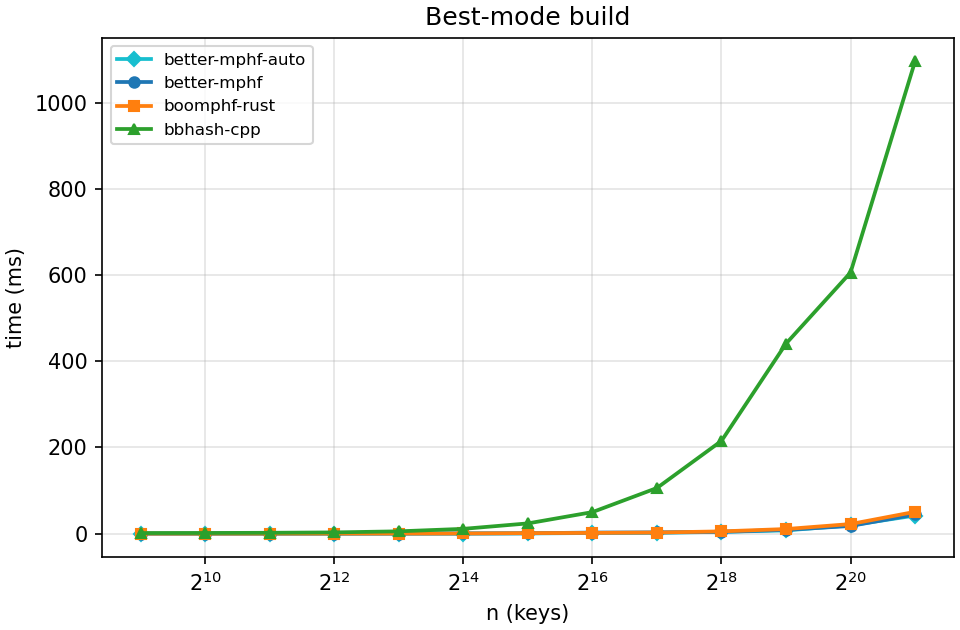
\includegraphics[width=\linewidth]{figures/best_mode_build.png}
\end{minipage}
\hfill
\begin{minipage}[t]{0.45\linewidth}
\centering
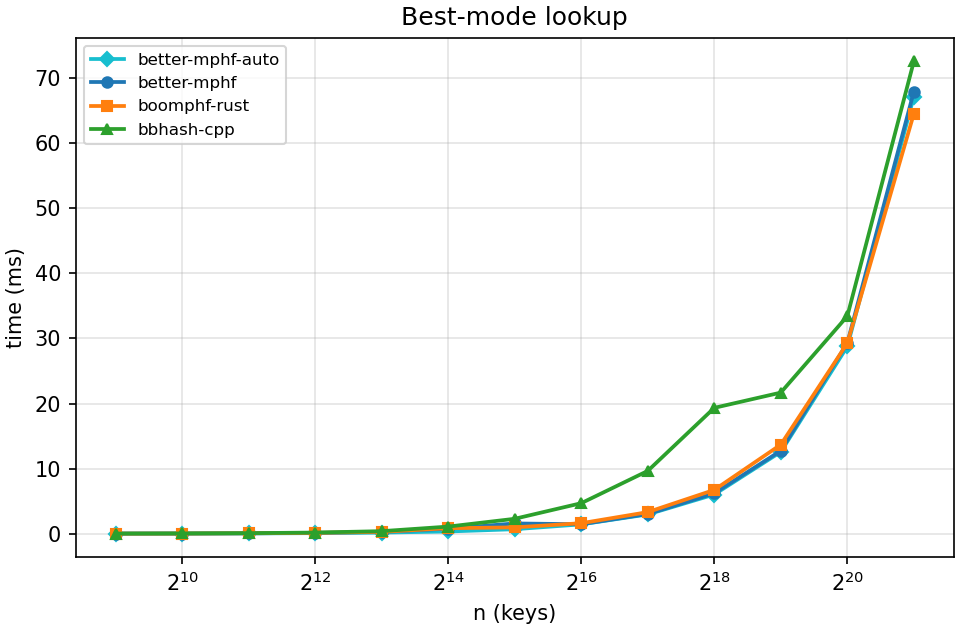
\includegraphics[width=\linewidth]{figures/best_mode_lookup.png}
\end{minipage}
\caption{Left: best-mode build. Right: best-mode lookup.}
\label{fig:best-mode}
\end{figure}
\FloatBarrier

\subsection{Auto-Gamma Results}
In the \PaperSeedCount{}-seed benchmark, auto was compared against the best fixed gamma for the same seed and input size (\PaperAutoComparisonCellCount{} comparison cells: $\PaperSeedCount$ seeds $\times$ $\PaperSizeCount$ sizes). Auto was better in \PaperAutoBuildBetterWins{} build cells and worse in \PaperAutoBuildWorseWins{}, with a median build slowdown of \PaperAutoBuildMedianSlowdownPct\% relative to best fixed. On lookup, auto was better in \PaperAutoLookupBetterWins{} cells and worse in \PaperAutoLookupWorseWins{}, with a median advantage of \PaperAutoLookupMedianAdvantagePct\%.

This makes auto a strong default when the goal is good lookup performance without hand-tuning $\gamma$. Auto is essentially tied with the best fixed gamma on build and is better on average for lookup.

\begin{figure}[!htbp]
\centering
\begin{minipage}[t]{0.45\linewidth}
\centering
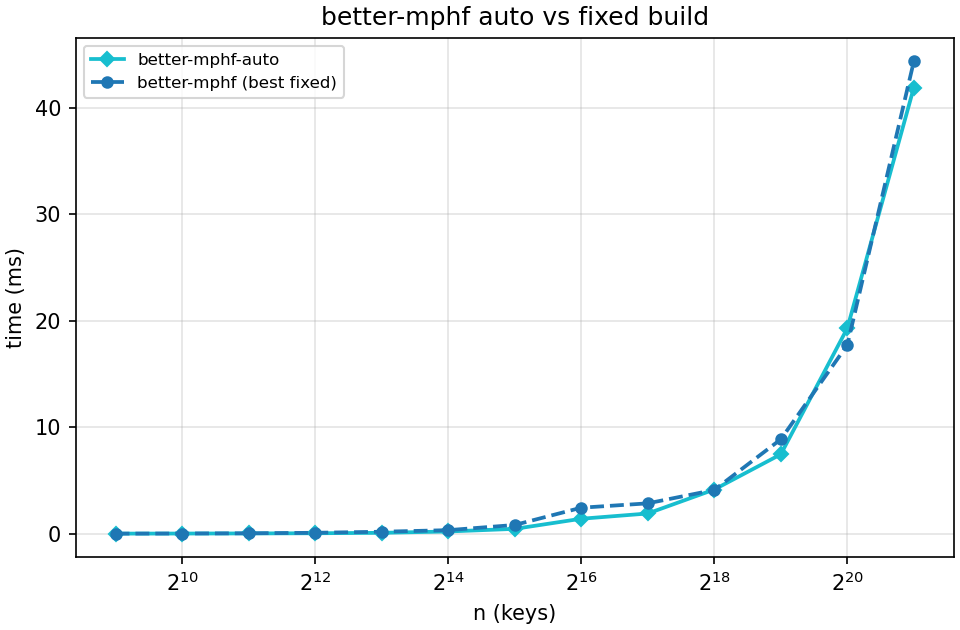
\includegraphics[width=\linewidth]{figures/better_auto_vs_fixed_build.png}
\end{minipage}
\hfill
\begin{minipage}[t]{0.45\linewidth}
\centering
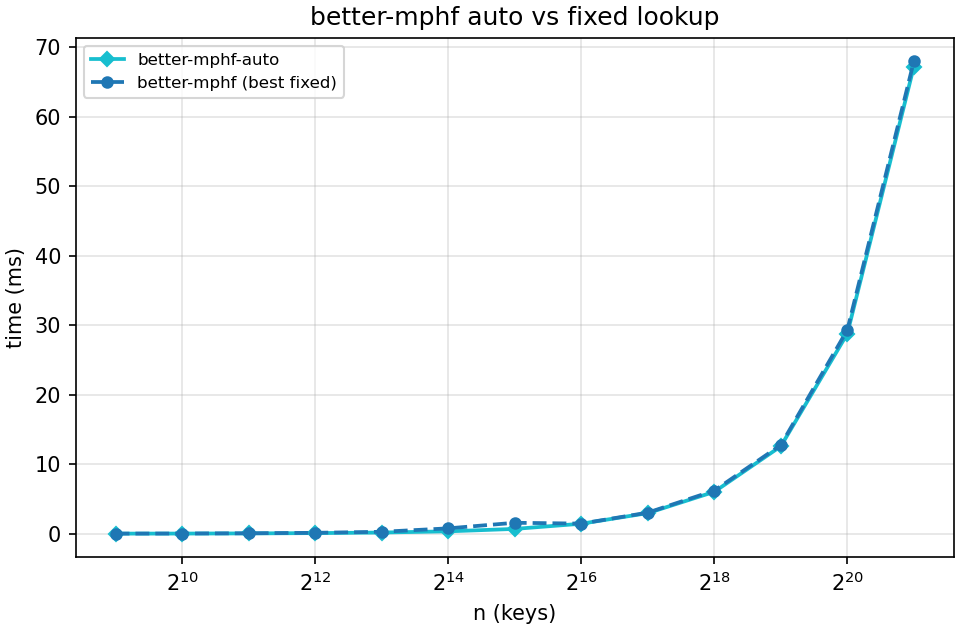
\includegraphics[width=\linewidth]{figures/better_auto_vs_fixed_lookup.png}
\end{minipage}
\caption{Left: \texttt{better-mphf-auto} build versus best fixed gamma. Right: \texttt{better-mphf-auto} lookup versus best fixed gamma.}
\label{fig:auto-vs-fixed}
\end{figure}
\FloatBarrier

\subsection{Per-Gamma View and Workload Sensitivity}
Figure~\ref{fig:gamma-grid} shows the fixed-gamma results in more detail. \texttt{better-mphf} performs best for medium to large $n$ values, especially in lookup. The weakest cells are concentrated at very small sizes.

\begin{figure}[!htbp]
\centering
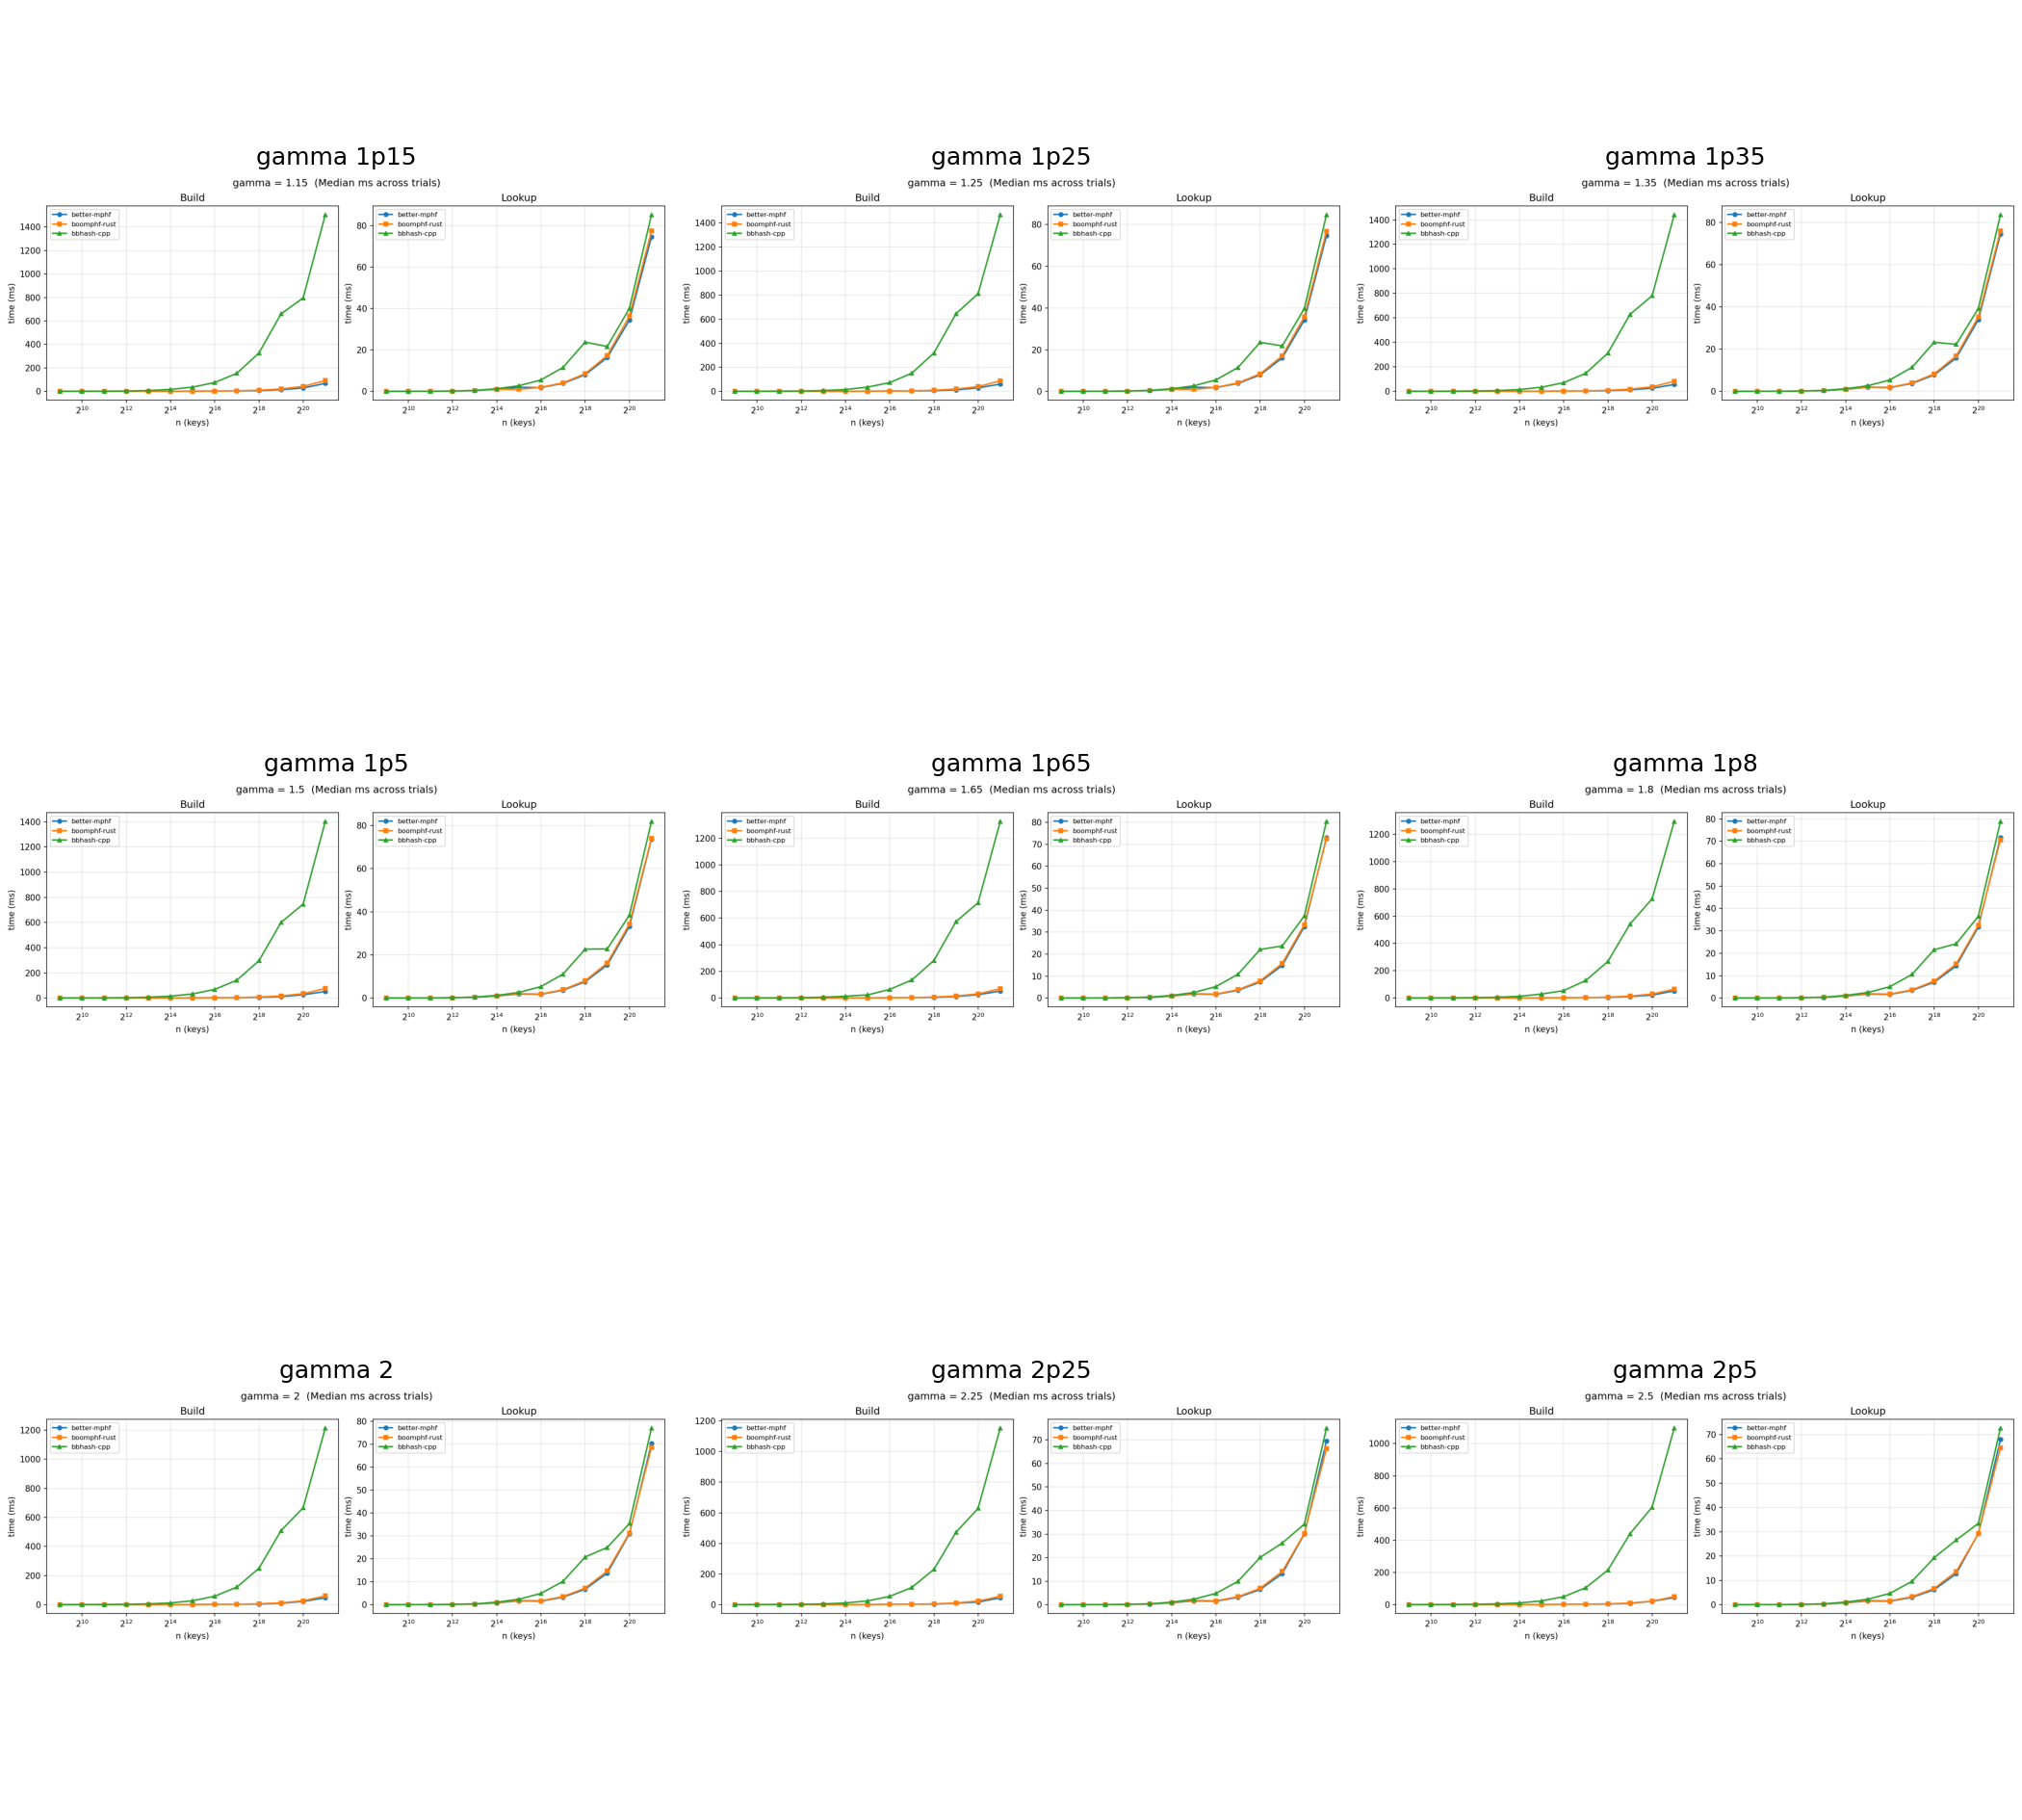
\includegraphics[width=\linewidth]{figures/gamma_grid_serial.png}
\caption{Per-gamma fairness plots from the \PaperSeedCount{}-seed benchmark.}
\label{fig:gamma-grid}
\end{figure}
\FloatBarrier

The fast-range comparison shows a clear pattern in the current data. In the \PaperCollapsedCellCount{}-cell view, build winners split \PaperFastRangeBuildMulSixtyFourWins/\PaperFastRangeBuildLowThirtyTwoWins/\PaperFastRangeBuildHighThirtyTwoWins{} among \texttt{mul64}/\texttt{low32}/\texttt{high32}, and lookup winners split \PaperFastRangeLookupMulSixtyFourWins/\PaperFastRangeLookupLowThirtyTwoWins/\PaperFastRangeLookupHighThirtyTwoWins{} among \texttt{mul64}/\texttt{low32}/\texttt{high32}. Relative to \texttt{low32}, \texttt{mul64} improves median build time by \PaperFastRangeMulSixtyFourBuildImprovePct\% and median lookup time by \PaperFastRangeMulSixtyFourLookupImprovePct\%, while \texttt{high32} improves build by \PaperFastRangeHighThirtyTwoBuildImprovePct\% but hurts lookup by \PaperFastRangeHighThirtyTwoLookupPenaltyPct\%. In this comparison, \texttt{mul64} is the strongest overall mode.

The key-distribution comparison tells a similar story. Lookup is very stable across tested modes: relative to multiplicative keys, the median lookup change stayed within about $\pm \PaperKeyLookupBoundPct\%$ for sequential, clustered, high-bit-heavy, and splitmix-random keys. Build is more workload-sensitive, and every tested alternative distribution was slower than multiplicative keys, with median slowdowns from \PaperKeyBuildShiftMinPct\% to \PaperKeyBuildShiftMaxPct\%. No distribution produced a failure mode.

\begin{figure}[!htbp]
\centering
\begin{minipage}[t]{0.49\linewidth}
\centering
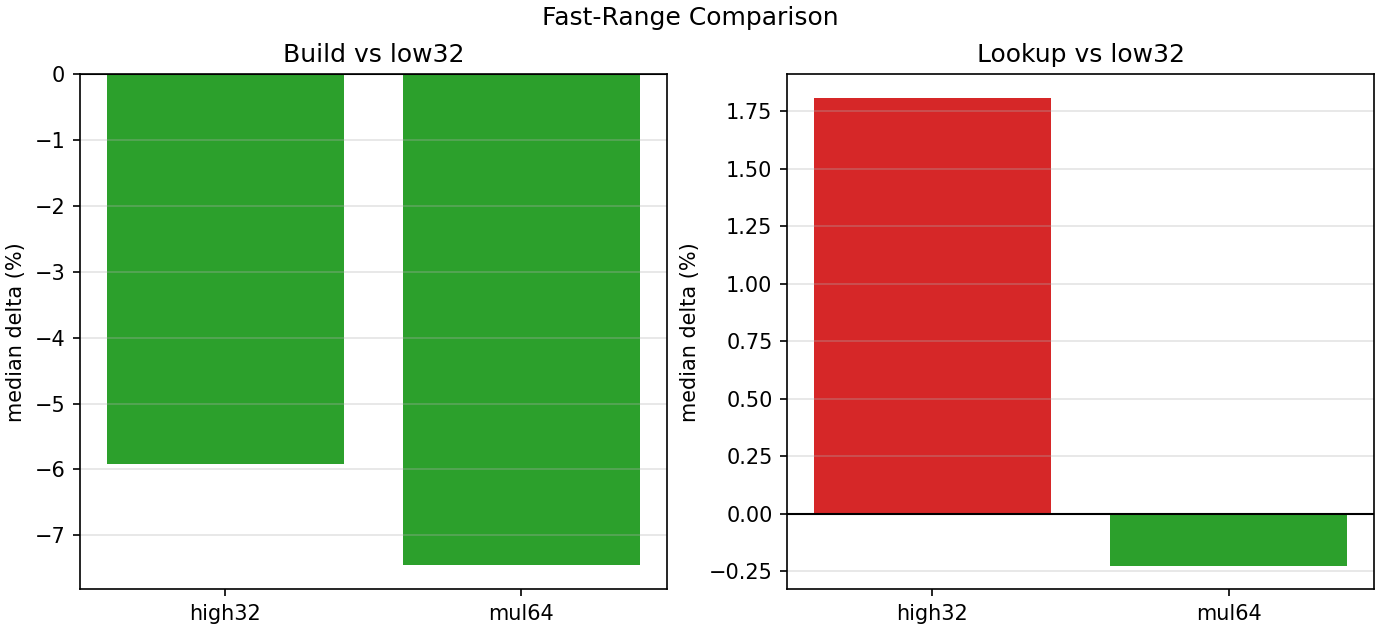
\includegraphics[width=\linewidth]{figures/fastrange_tradeoff.png}
\end{minipage}
\hfill
\begin{minipage}[t]{0.49\linewidth}
\centering
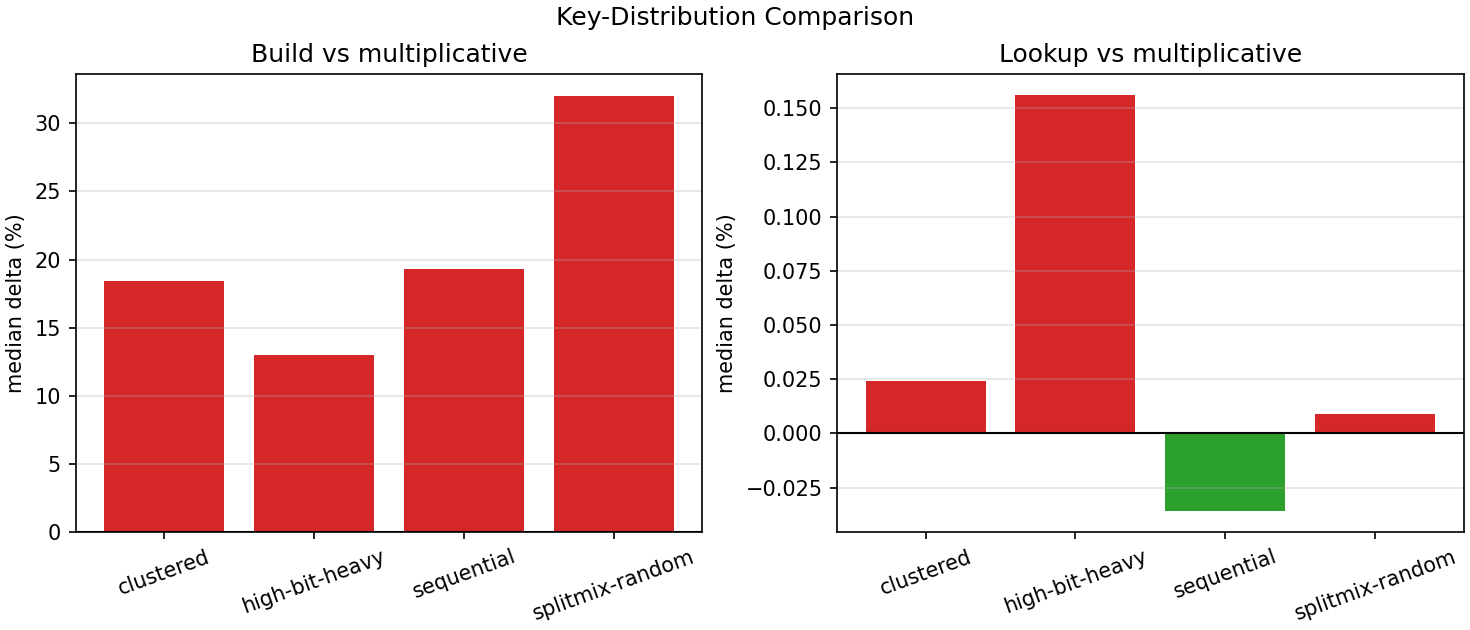
\includegraphics[width=\linewidth]{figures/keymode_tradeoff.png}
\end{minipage}
\caption{Left: fast-range comparison. Right: key-distribution comparison.}
\label{fig:tradeoff-panels}
\end{figure}
\FloatBarrier

\subsection{Seed Robustness}
Seed sensitivity is the main weakness of the current builder. In the \PaperSeedCount{}-seed benchmark, the worst/best build-time ratio across seeds has a median of $\PaperSeedRatioMedianX\times$ and a maximum of $\PaperSeedRatioMaxX\times$. At $n = \PaperSeedExampleN$, the fixed-gamma benchmark gives representative per-gamma ranges: at $\gamma = \PaperSeedExampleGammaLow$, best/median/worst across \PaperSeedCount{} seeds is \PaperSeedLowBestMs/\PaperSeedLowMedianMs/\PaperSeedLowWorstMs ms; at $\gamma = \PaperSeedExampleGammaHigh$, it is \PaperSeedHighBestMs/\PaperSeedHighMedianMs/\PaperSeedHighWorstMs ms.

This spread shows why one fixed seed is not enough for evaluation. A single unlucky seed can make a stable implementation look much worse than it really is, which is why the paper relies on multi-seed results.

\begin{figure}[!htbp]
\centering
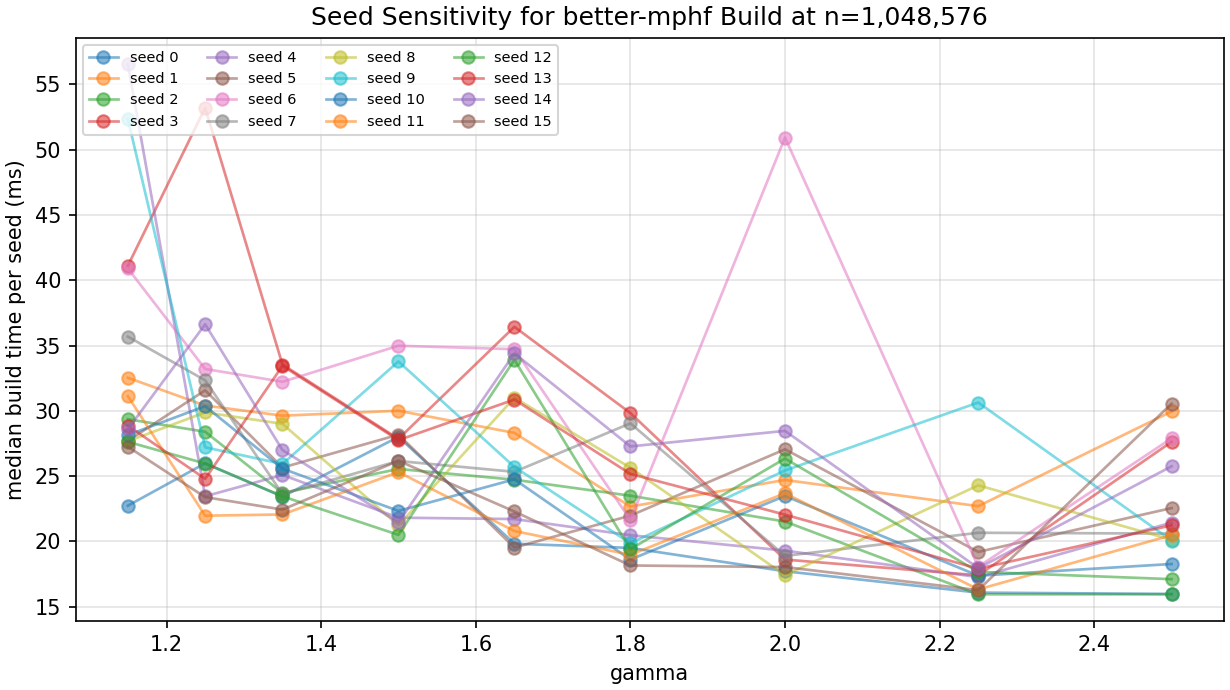
\includegraphics[width=0.8\linewidth]{figures/seed_variance_1m_build.png}
\caption{Seed sensitivity for \texttt{better-mphf} build at $n = \PaperSeedExampleN$.}
\label{fig:seed}
\end{figure}
\FloatBarrier

\section{Conclusion}
The most important outcome is that the Rust implementation now meets the intended static-workload profile reasonably well. Lookup is the strongest phase: in the seed-median view, \texttt{better-mphf} wins \PaperMedianLookupBetterWins{} of \PaperCollapsedCellCount{} lookup cells overall, and \PaperLargeLookupBetterWins{} of \PaperLargeCellCount{} cells at $n \ge \PaperLargeNThreshold$, where input sizes are large enough for timer noise not to dominate. Construction is competitive for medium and large inputs: \PaperMedianBuildBetterWins{} of \PaperCollapsedCellCount{} build cells overall, and \PaperLargeBuildBetterWins{} of \PaperLargeCellCount{} at $n \ge \PaperLargeNThreshold$. At the small-$n$ values, there is a lot more noise and the wins are less meaningful.

The remaining problem is that unlucky seeds can increase construction time. The next focus should be reducing seed-dependent variance while keeping strict Poisson acceptance unchanged so that level count and lookup quality do not regress.

\begin{thebibliography}{9}

\bibitem{sea2017}
Antoine Limasset, Guillaume Rizk, Rayan Chikhi, and Pierre Peterlongo,
\emph{Fast and Scalable Minimal Perfect Hashing for Massive Key Sets},
16th International Symposium on Experimental Algorithms (SEA), 2017.

\bibitem{boomphf-rust}
\texttt{boomphf} Rust crate, \url{https://crates.io/crates/boomphf}.

\bibitem{bbhash-cpp}
BBHash C++ library, \url{https://github.com/rizkg/BBHash}.

\bibitem{lemire2019}
Daniel Lemire,
\emph{Fast Random Integer Generation in an Interval},
ACM Transactions on Modeling and Computer Simulation, 29(1), 2019.

\end{thebibliography}

\end{document}